\documentclass[]{article}

% Imported Packages
%------------------------------------------------------------------------------
\usepackage{amssymb}
\usepackage{amstext}
\usepackage{amsthm}
\usepackage{amsmath}
\usepackage{enumerate}
\usepackage{fancyhdr}
\usepackage[margin=1in]{geometry}
\usepackage{graphicx}
\usepackage{extarrows}
\usepackage{setspace}
\usepackage{graphicx}
\graphicspath{ {./asset/} }
%\usepackage{extarrows}
%\usepackage{setspace}
%\usepackage{xcolor}
\usepackage{color}
%------------------------------------------------------------------------------

% Header and Footer
%------------------------------------------------------------------------------
\pagestyle{plain}  
\renewcommand\headrulewidth{0.4pt}                                      
\renewcommand\footrulewidth{0.4pt}                                    
%------------------------------------------------------------------------------

% Title Details
%------------------------------------------------------------------------------
\title{Deliverable \#1 Template}
\author{SE 3A04: Software Design II -- Large System Design}
\date{}                               
%------------------------------------------------------------------------------

% Document
%------------------------------------------------------------------------------
\begin{document}

\maketitle	

\section{Introduction}
\label{sec:introduction}
% Begin Section

The following document is dedicated to showcasing the requirements of the taxi carpool app requested by a local taxi company. The app is dedicated to make rides cheaper and more convenient for their riders. This app is also meant to be a long-term project for the company, meaning this SRS is a living document which has the possibility of changing in the future. This document will explain the important stakeholders involved, requirements and viewpoints of each while also explaining the main functions of the app.

\subsection{Purpose}
\label{sub:purpose}
% Begin SubSection
This SRS is meant for developers, stakeholders and direct players in the planning and development of the app and should be understandable for all those involved. This SRS will further break down the functionalities, constraints, use cases and overall design of the project in further detail. 

% End SubSection

\subsection{Scope}
\label{sub:scope}
% Begin SubSection
To develop this project the production of the main taxi request and offer app called TaxiCarPool, the Conversation Prompt Generator and a variety of databases will have to be produced. There will not be a need to produce a payment system into the app as this will be handled by the taxi company payment systems. The project will only project the cost of the ride but will not handle the payments as it is not part of the app’s main functionality.
\newline \newline
The TaxiCarPool app will perform the main functions of the app. This will include allowing users to request a carpool taxi, receive a list of possible rides to select and allow current rides to allow carpooling in their car. This product’s objective is to perform the main functions of matchmaking users to a carpool to save money. 
\newline \newline
The Conversation Prompt Generator will randomly generate a conversation starter for the riders to use based on their profile. Their profile will specify if they want to use this feature and if so, what they are interested in. The generator will not be forced upon any of the users and can be switched off if desired. The goal of this product is to create a friendly environment when carpooling with others that one may not know. This function is mostly dedicated to benefit those who are carpooling to a further distance.
\newline \newline
The creation of a database will hold all the necessary information for the app to function, making it easily accessible and manageable. The information being stored can range from user information; name, email, phone number, to riding history, to preferences of taxi times, models, or other passengers. 
% End SubSection

\subsection{Definitions, Acronyms, and Abbreviations}
\label{sub:definitions_acronyms_and_abbreviations}
% Begin SubSection
BE: Business Event is something that occurs between the client/stakeholder and the system. 
\newline \newline
SRS: Software Requirements Specification is a document that explains the requirements of the software being developed.
\newline \newline
VP: Viewpoint, often in reference to a stakeholder/client interested in the system and how they view the business event.
% End SubSection

\subsection{References}
\label{sub:references}
% Begin SubSection
\begin{itemize}
	\item Johns, K. (2022, July 7). Why design is the most important factor in a mobile app development?: ISHIR- mobile application development company india. ISHIR. Retrieved February 11, 2023, from https://www.ishir.com/blog/9633/why-design-is-the-most-important-factor-in-a-mobile-app-development.htm 
	\item Schoenfelder, N. (n.d.). What are good latency \& ping speeds? Graphical Network Monitoring and Troubleshooting. Retrieved February 11, 2023, from https://www.pingplotter.com/wisdom/article/is-my-connection-good 
	\item statcounter. (n.d.). Mobile Operating System Market Share Worldwide. StatCounter Global Stats. Retrieved February 11, 2023, from https://gs.statcounter.com/os-market-share/mobile/worldwide 
	\item UGEM. (2020, June 15). What are the core features of Minimalist app design? UGEM. Retrieved February 11, 2023, from https://ugem.design/blog/minimal-app-design 
	\item Yee, J. (n.d.). Introduction to canadian digital accessibility laws. Accessibility.com: Empowering digital accessibility for businesses. Retrieved February 11, 2023, from https://www.accessibility.com/blog/introduction-to-canadian-digital-accessibility-laws 
\end{itemize}
% End SubSection

\subsection{Overview}
\label{sub:overview}
% Begin SubSection
This SRS is structured to first give background information about the app. This will include how the app will interface with the taxi companies, along with the general functionalities and assumptions that are being made. The document will then follow with showcasing one of the main business events and its related use cases. This will explain how the main function will work across different scenarios and stakeholders in a visual manner. This will be further expanded upon in more detail throughout the document. It will include more business events with a variety of viewpoints and scenarios for both the function shown in the use case diagram and other main function of the project. This document will conclude by explaining the non-functional requirements involving presentation, performance, usability, security, and maintainability notes of the project.
% End SubSection

% End Section

\section{Overall Description}
\label{sec:overall_description}
% Begin Section

\begin{itemize}
	\item This section of the SRS should describe the general factors that affect the product and its requirements. 
	\item It does not state specific requirements.
	\item It provides a \emph{background} for those requirements and makes them easier to understand.
\end{itemize}


\subsection{Product Perspective}
\label{sub:product_perspective}
% Begin SubSection

\begin{enumerate}[a)]
	\item The product being developed is an Android application which empowers the ability to book carpool via a user-friendly interface using a taxi company. The application will securely store customer personal information such as carpool request histories, and personal data inputted by the user. The product is not self-contained since its functionality depends heavily on the taxi service provider. There are several out-of-scope concerns such as: driver\textquotesingle s information input (profile, shift, locations, etc.) and payment processing.
	\item The general interaction can be visualized as follows: 
	\begin{center}
		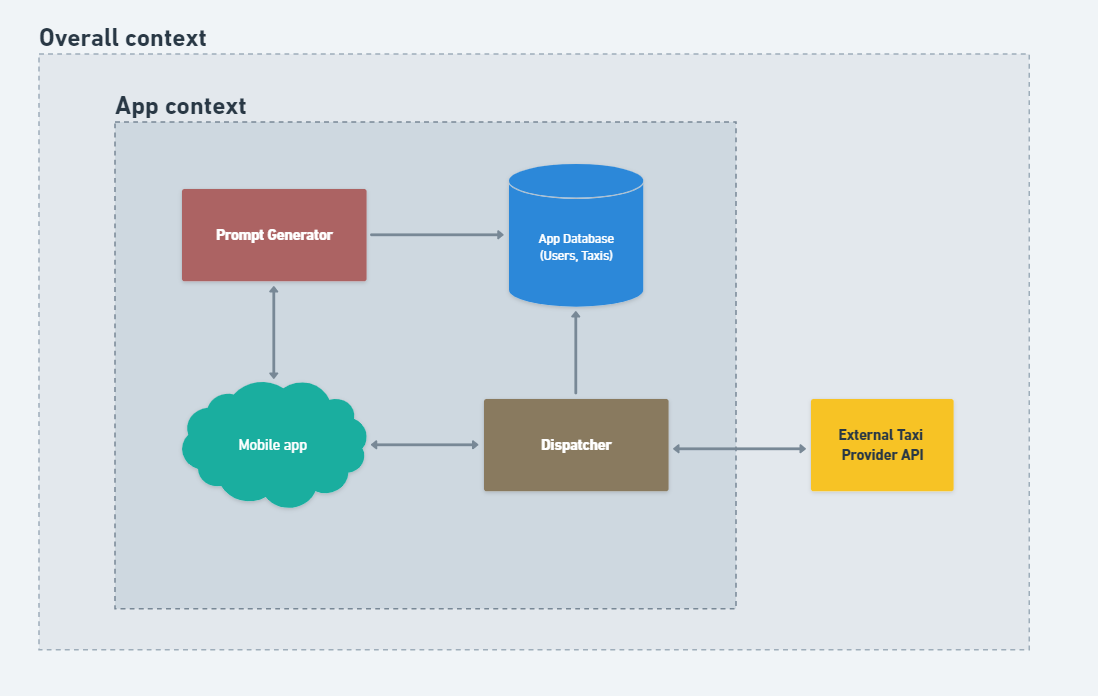
\includegraphics[scale=0.5]{app-context.png}
	\end{center}
\end{enumerate}

% End SubSection

\subsection{Product Functions}
\label{sub:product_functions}
% Begin SubSection
	\begin{center}
		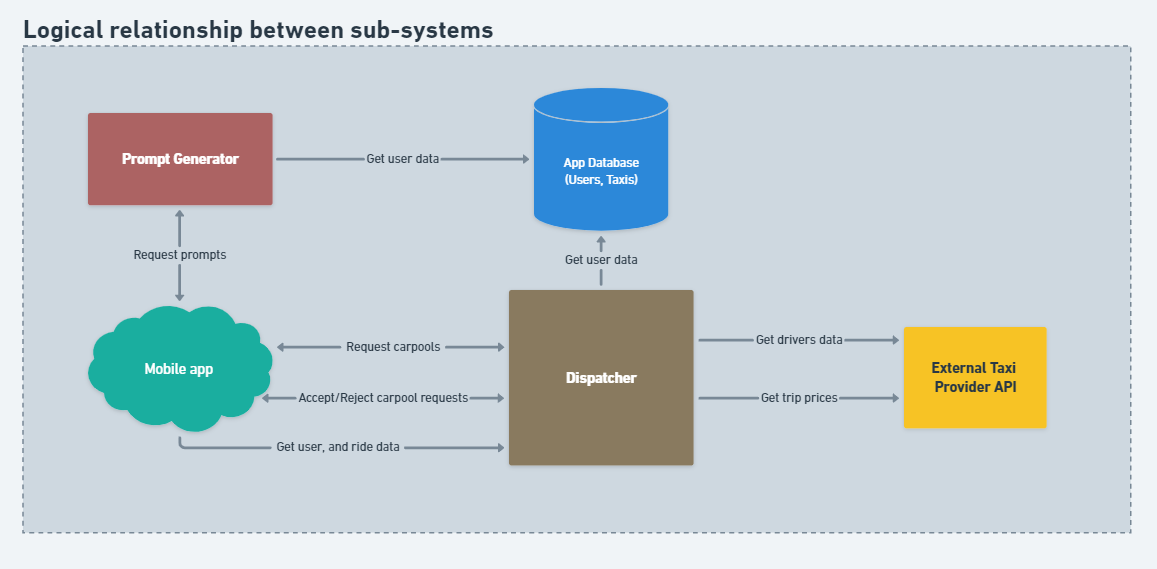
\includegraphics[scale=0.5]{subsys-relationship.png}
	\end{center}

\begin{enumerate}[a)]
	\item The app will be able to book taxi.

	\begin{itemize}
		\item Able to communicate with taxi\textquotesingle s service API.
		\item Able to handle and display taxi data correctly.	
	\end{itemize}
	\item The app be able to handle carpool scheduling and coordination.
	\begin{itemize}
		\item Able to plan the most optimal route and let the driver follow the calculated route.
	\end{itemize}
	\item The app be able to display the estimate time-of-arrival (ETA) of taxis.
	\begin{itemize}
		\item Able to calculate ETA in real-time
	\end{itemize}
	\item The app be able to input the taxi\textquotesingle s unique identifier via the mobile app.
\end{enumerate}

% End SubSection

\subsection{User Characteristics}
\label{sub:user_characteristics}
% Begin SubSection

\begin{enumerate}[a)]
	\item Riders
	\begin{itemize}
		\item Riders are users who use the app to request car pool.
		\item Riders can be anyone from any background of tech-expertise
		\item Riders are expected to:
		\begin{itemize}
			\item Input personal information only a few times.
			\item Have stable and highly available mobile internet connection.
		\end{itemize}
		
		\item Riders might be interested one or more following characteristics of the app:
		\begin{itemize}
			\item User interface and experience of navigating the mobile app.
			\item Realtime taxi information display (ETA, location, route, …)
			\item Ease of taxi booking, and check-in.  
		\end{itemize}
	\end{itemize}
	
	\item Taxi Drivers
	\begin{itemize}
		\item Drivers are users who drive and operate taxis, fulfill carpool requests, and ensure the safety of the riders.
		\item Drivers must be registered with the taxi service and from any background of tech-expertise.  
		\item Drivers are expected to have stable and highly available mobile internet connection.
		\item Drivers might be interested one or more following characteristics of the app:
		\begin{itemize}
			\item Accuracy display of real-time pick-up and drop-off information.
			\item Accuracy of aggregating and storing of rides information (since it ties directly to their performance).
			\item Accuracy display of user\textquotesingle s profile summarization.
			\item User interface and experience of navigating the mobile app.
			\item Ease of accepting/ rejecting rides.
		\end{itemize}

	\end{itemize}

\end{enumerate}

% End SubSection

\subsection{Constraints}
\label{sub:constraints}
% Begin SubSection
\begin{enumerate}[a)]
	\item \textbf{Geographical}: The app can only operate on the land which the taxi service operate.
	\item \textbf{Technological}: App must be integrated with softwares that the taxi service provider uses.
	\item \textbf{Fare Determination}: Since the app does\textquotesingle t support payment processing directly, the fare has to be determined and processed through the taxi service provider.
	\item \textbf{Data Privacy Regulation}: Data which transmits and stored within the app needs to be processed in a way which complies with the data protection act.

\end{enumerate}

% End SubSection

\subsection{Assumptions and Dependencies}
\label{sub:assumptions_and_dependencies}
% Begin SubSection


\begin{enumerate}[a)]
	\item Assumptions

	\begin{itemize}
		\item Drivers information are provided by the taxi provider (driver profile and shift).
		\item The taxi provider has dedicated API which provide real-time data on driver\textquotesingle s availability.
		\item The taxi provider determines trip prices.
		\item Payment processing is external and not under the scope of the application.

	\end{itemize}

	\item Many problems may occur when the following assumptions failed to hold:
	\begin{itemize}
		\item If trip prices are not determined by the taxi service provider, additional calculations must be performed to find fare fees after each trip.
		\item If drivers data are stored and handled within the context of the app, additional mechanism must be provided for drivers to update their information. In addition, driver\textquotesingle s data storage must comply with the Canadian Data Protection Act. 


	\end{itemize}
\end{enumerate}
% End SubSection

\subsection{Apportioning of Requirements}
\label{sub:apportioning_of_requirements}
% Begin SubSection

\begin{enumerate}[a)]
	\item \textbf{Technological}: Some specific technilogical requirements (Database type, Integration with taxi provider, etc...) have to be delayed untill the implementation phase.
	\item Non-function Requiremens such as UI,UX, or performance can be finetuned when the app is being implemented or after release.
\end{enumerate}

% End SubSection

% End Section
\section{Use Case Diagram}
\label{sec:use_case_diagram}
% Begin Section
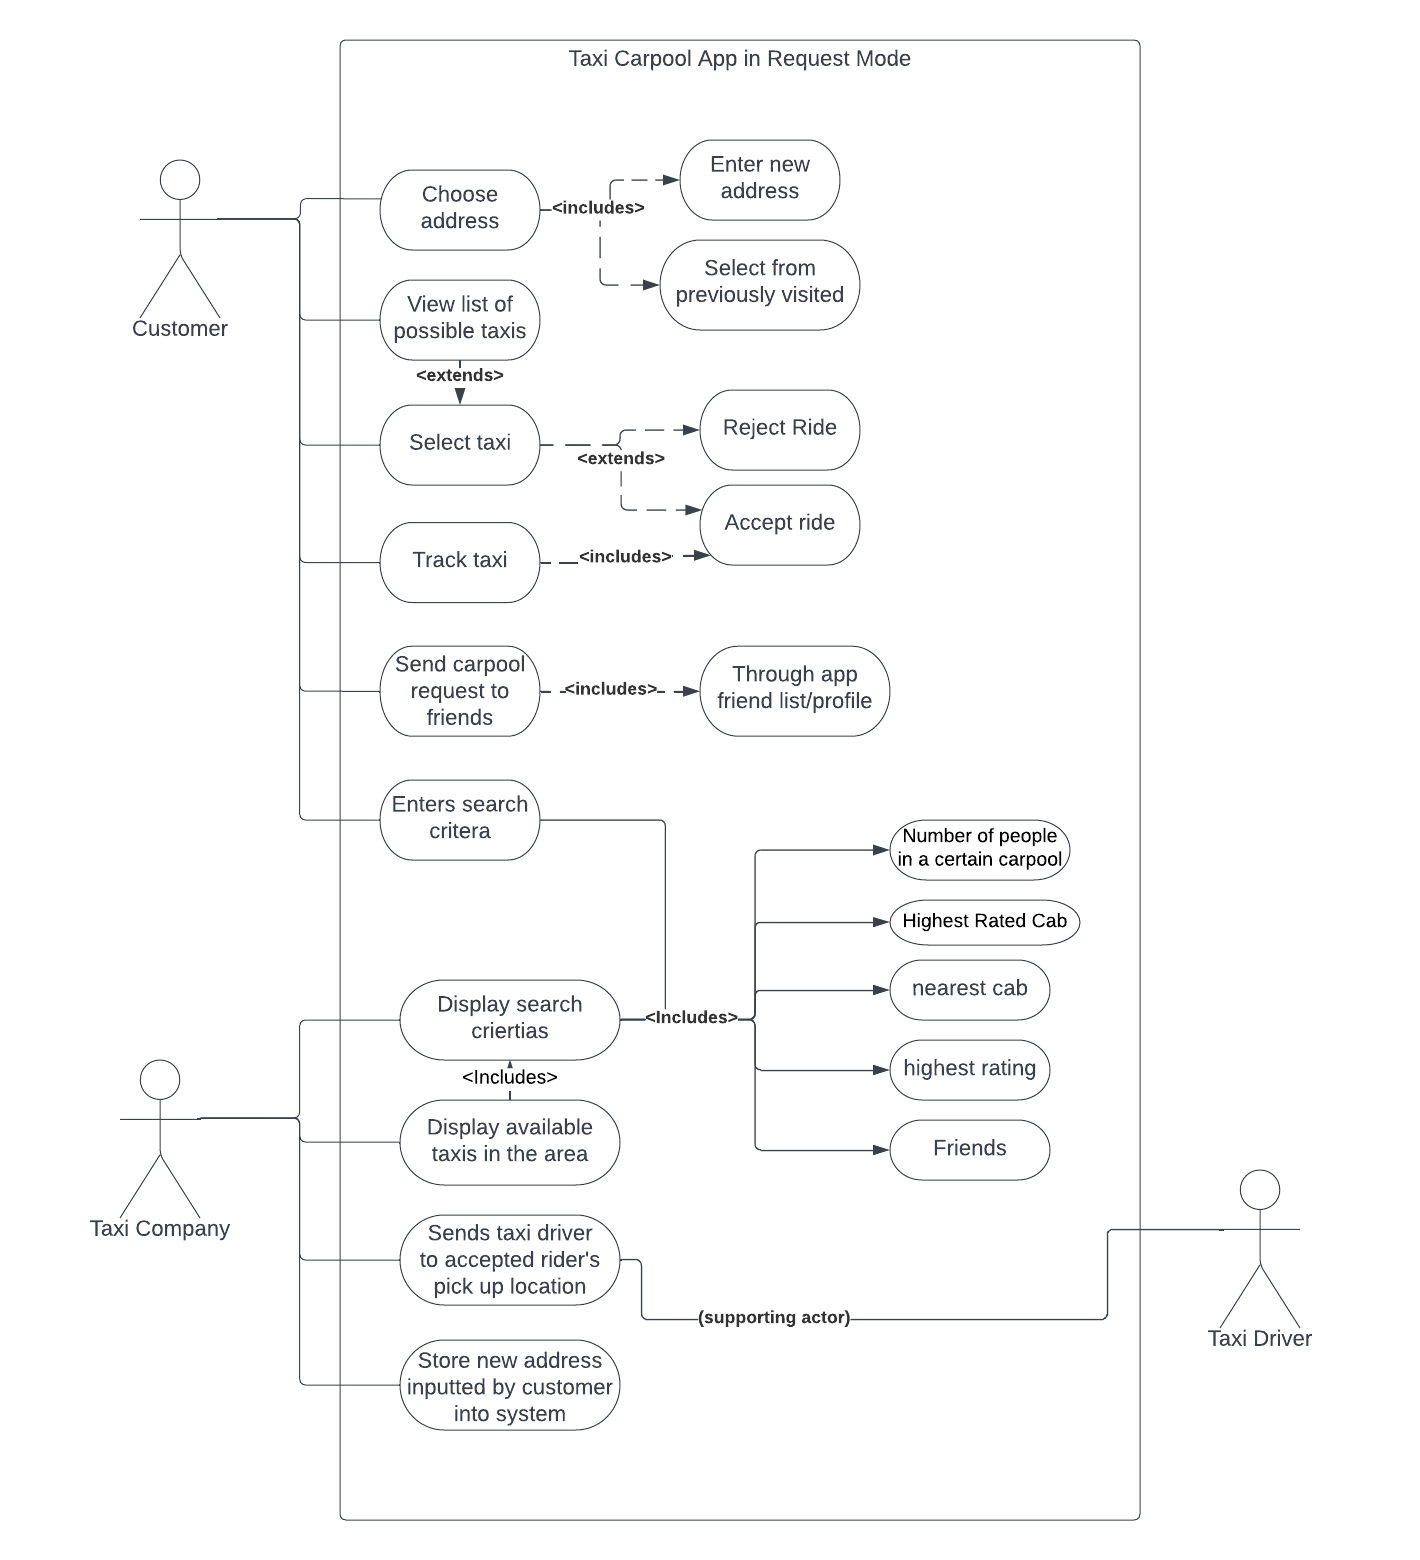
\includegraphics[scale = 0.8]{Use_Case_Diagram.png}

%In this section, select the most important Business Event that your system responds to and give its use case diagram.  Only one use case diagram is needed.  Give a brief textual description of the use case without repeating what is in the scenarios of the corresponding Business Event.

%
%
%
%This section should provide a use case diagram for your application. 
%\begin{enumerate}[a)]
%	\item Each use case appearing in the diagram should be accompanied by a text description. 
%\end{enumerate}
%% End Section

\section{Highlights of Functional Requirements}
\label{sec:functional_requirements}
% Begin Section
\begin{itemize}
	\item Specify the "use cases" organized by Business Event. (The Global Scenario is what you might think of as a use case). Be sure to consider Business Events that aren't just triggered by users with goals (e.g. something happens in the environment that your system needs to respond to)
	\item Your focus should be on what the system needs to do, not how to do it. Specify it in enough detail that it clearly specifies what needs to be accomplished, but not so detailed that you start programming or making design decisions.
	\item Keep the length of each use case (Global Scenario) manageable. If it's getting too long, you need to condense your steps and give a name to what's accomplished by that sequence of steps. (e.g. "Authenticate user" in one line, instead of a list of steps of how to; that's a design decision anyways)
	\item You are \emph{not} specifying a complete and consistent set of functional requirements here. (i.e. you are providing them in the form of use cases/global scenarios, not a refined list). For the purpose of this project, you do not need to reduce them to a list; the global scenarios format is all you need.
\end{itemize}
	Below, we organize by Business Event.
	\begin{enumerate}[{BE}1.]
		\item Business Event name
		\begin{enumerate}[{VP1}.1]
			\item Viewpoint name \newline
			\noindent\fbox{%
				\parbox{0.5\textwidth}{%
					\begin{itemize}
						\item {\bf $S_{1}$:} Initial response of the system to the Business Event
						\item {\bf $E_{1}$:}  Reaction of the environment to $S_{1}$
						\item {\bf $S_{2}$:}  Response of the system to $E_{1}$
						\item {\bf $E_{2}$:}  Reaction of the environment to $S_{2}$
						\item[] $\cdots$
						\item {\bf $S_{n}$:}  Response of the system to $E_{(n-1)}$
						\item {\bf $E_{n}$:}  Reaction of the environment to $E_{(n-1)}$
						\item {\bf $S_{(n+1)}$:} Final response of the system concluding its function regarding the Business Event
					\end{itemize}
				}%
			}
			\item Viewpoint name\newline
			\noindent\fbox{%
				\parbox{0.5\textwidth}{%
					\begin{itemize}
						\item {\bf $S_{1}$:} Initial response of the system to the Business Event
						\item {\bf $E_{1}$:}  Reaction of the environment to $S_{1}$
						\item {\bf $S_{2}$:}  Response of the system to $E_{1}$
						\item {\bf $E_{2}$:}  Reaction of the environment to $S_{2}$
						\item[] $\cdots$
						\item {\bf $S_{k}$:}  Response of the system to $E_{(k-1)}$
						\item {\bf $E_{k}$:}  Reaction of the environment to $E_{(k-1)}$
						\item {\bf $S_{(k+1)}$:} Final response of the system concluding its function regarding the Business Event
					\end{itemize}
				}%
			}
			\item \dots
			\item \dots
			\item \dots
			\item[\dots]
		\end{enumerate}	
		\item[] {\bf Global Scenario of {\it Business Event Name}:} It is the scenario corresponding to the integration of all the above scenarios from the different Viewpoints of the Business Event BE1.\newline
		\noindent\fbox{%
			\parbox{0.5\textwidth}{%
				\begin{itemize}
					\item {\bf $S_{1}$:} Initial response of the system to the Business Event
					\item {\bf $E_{1}$:}  Reaction of the environment to $S_{1}$
					\item {\bf $S_{2}$:}  Response of the system to $E_{1}$
					\item {\bf $E_{2}$:}  Reaction of the environment to $S_{2}$
					\item[] $\cdots$
					\item {\bf $S_{m}$:}  Response of the system to $E_{(m-1)}$
					\item {\bf $E_{m}$:}  Reaction of the environment to $E_{(m-1)}$
					\item {\bf $S_{(m+1)}$:} Final response of the system concluding its function regarding the Business Event
				\end{itemize}
			}%
		}	
		%\end{enumerate}
		\item Business Event name
		\begin{enumerate}[{VP1}.1]
			\item Viewpoint name \newline
			\noindent\fbox{%
				\parbox{0.5\textwidth}{%
					\begin{itemize}
						\item {\bf $S_{1}$:} Initial response of the system to the Business Event
						\item {\bf $E_{1}$:}  Reaction of the environment to $S_{1}$
						\item {\bf $S_{2}$:}  Response of the system to $E_{1}$
						\item {\bf $E_{2}$:}  Reaction of the environment to $S_{2}$
						\item[] $\cdots$
						\item {\bf $S_{n'}$:}  Response of the system to $E_{(n'-1)}$
						\item {\bf $E_{n'}$:}  Reaction of the environment to $E_{(n'-1)}$
						\item {\bf $S_{(n'+1)}$:} Final response of the system concluding its function regarding the Business Event
					\end{itemize}
				}%
			}
			\item Viewpoint name\newline
			\noindent\fbox{%
				\parbox{0.5\textwidth}{%
					\begin{itemize}
						\item {\bf $S_{1}$:} Initial response of the system to the Business Event
						\item {\bf $E_{1}$:}  Reaction of the environment to $S_{1}$
						\item {\bf $S_{2}$:}  Response of the system to $E_{1}$
						\item {\bf $E_{2}$:}  Reaction of the environment to $S_{2}$
						\item[] $\cdots$
						\item {\bf $S_{k'}$:}  Response of the system to $E_{(k'-1)}$
						\item {\bf $E_{k'}$:}  Reaction of the environment to $E_{(k'-1)}$
						\item {\bf $S_{(k'+1)}$:} Final response of the system concluding its function regarding the Business Event
					\end{itemize}
				}%
			}
			\item \dots
			\item \dots
			\item \dots
			\item[\dots]
		\end{enumerate}	
		\item[] {\bf Global Scenario of {\it Business Event Name}:} It is the scenario corresponding to the integration of all the above scenarios from the different Viewpoints of the Business Event BE2.\newline
		\noindent\fbox{%
			\parbox{0.5\textwidth}{%
				\begin{itemize}
					\item {\bf $S_{1}$:} Initial response of the system to the Business Event
					\item {\bf $E_{1}$:}  Reaction of the environment to $S_{1}$
					\item {\bf $S_{2}$:}  Response of the system to $E_{1}$
					\item {\bf $E_{2}$:}  Reaction of the environment to $S_{2}$
					\item[] $\cdots$
					\item {\bf $S_{m'}$:}  Response of the system to $E_{(m'-1)}$
					\item {\bf $E_{m'}$:}  Reaction of the environment to $E_{(m'-1)}$
					\item {\bf $S_{(m'+1)}$:} Final response of the system concluding its function regarding the Business Event
				\end{itemize}
			}%
		}		
	\end{enumerate}

%End Section

\section{Non-Functional Requirements}
\label{sec:non-functional_requirements}

% Begin Section
\subsection{Look and Feel Requirements}
\label{sub:look_and_feel_requirements}
% Begin SubSection

\subsubsection{Appearance Requirements}
\label{ssub:appearance_requirements}
% Begin SubSubSection
\begin{enumerate}[{LF-A}1. ]
	\item The colour scheme of the application must match the branding colours of the company \\
	{\bf Rationale:} For marketing purposes, the colour scheme within the app need to match the branding colours of the company so the brand becomes well-recognized and there is no confusion among users about the brand.
\end{enumerate}
% End SubSubSection

\subsubsection{Style Requirements}
\label{ssub:style_requirements}
% Begin SubSubSection
\begin{enumerate}[{LF-S}1. ]
	\item The app must have an attractive, responsive UI \\
	{\bf Rationale:} Users are more likely to use and come back to attractive, responsive mobile apps which helps increase the user base and branding power of the app (Johns, 2022). 
	\item The app must have a minimalist design \\
	{\bf Rationale:} Minimalist designed mobile applications have faster loading times, easier navigation within the app, less maintenance and time spent on design/frontend and allow businesses to more clearly give messages to users within the application (UGEM, 2020).
\end{enumerate}
% End SubSubSection

% End SubSection

\subsection{Usability and Humanity Requirements}
\label{sub:usability_and_humanity_requirements}
% Begin SubSection

\subsubsection{Ease of Use Requirements}
\label{ssub:ease_of_use_requirements}
% Begin SubSubSection
\begin{enumerate}[{UH-EOU}1. ]
	\item The product must be easy to use for people aged 18 years or older \\
	{\bf Rationale:} The intended audience of this application is adults who need to carpool, so anyone 18 or older must find the app easy to understand and use. People under this age may use the app but most likely their rides would be booked by parents/guardians, so the focus is on this age range.
	\item The user must not encounter any unclear prompts from which they do not know how to proceed \\
	{\bf Rationale:} If the app is prompting the user to do something, that prompt must be clear and easy to understand so it is easy for the user to use the app.
	\item The user must not encounter any errors while using the app, and if they do, what to do next must be clear \\
	{\bf Rationale:} The app must not show the user any errors while they are using it to prevent confusion and to make the app easy to use. On the chance an error does appear to the user, it must be clear on what the user has to do next to remove the error or continue. If the error is generic and confusing to understand, the app is no longer easy to use and leaves the user in confusion.
\end{enumerate}
% End SubSubSection

\subsubsection{Personalization and Internationalization Requirements}
\label{ssub:personalization_and_internationalization_requirements}
% Begin SubSubSection
\begin{enumerate}[{UH-PI}1. ]
	\item The product will operate in both English and French and the user will be able to set their preferred language \\
	{\bf Rationale:} The app will be available only in Canada, so it needs to contain support for both the national languages of Canada and allow the user to choose their preferred language
	\item The product will allow the user to set their preference for dark mode and light mode \\
	{\bf Rationale:} To make the app more personal, users must be able to customize the appearance to their liking. Its important for users to enjoy the appearance of the app so allowing them to personalize dark mode or light mode will help contribute to that.
\end{enumerate}
% End SubSubSection

\subsubsection{Learning Requirements}
\label{ssub:learning_requirements}
% Begin SubSubSection
\begin{enumerate}[{UH-L}1. ]
	\item The product must be able to be used immediately, with no learning curve required to learn how to effectively use the app. \\
	{\bf Rationale:} Mobile apps designed for general users should have no learning curve. Upon using the app for the first time, the app should be designed in such a way that the user immediately knows how to use it. If users take a while to learn how to effectively use the app, they will not come back to it.
\end{enumerate}
% End SubSubSection

\subsubsection{Understandability and Politeness Requirements}
\label{ssub:understandability_and_politeness_requirements}
% Begin SubSubSection
\begin{enumerate}[{UH-UP}1. ]
	\item The product must use symbols and language that are naturally understandable to the general Canadian population \\
	{\bf Rationale:} The app is aimed to be used by anyone in Canada, so the symbols and language used must be understandable by the general Canadian population. Using symbols and language or slang that is specific to a certain group or culture would make the app hard to understand for some of the target users.
\end{enumerate}
% End SubSubSection

\subsubsection{Accessibility Requirements}
\label{ssub:accessibility_requirements}
% Begin SubSubSection
\begin{enumerate}[{UH-A}1. ]
	\item The product must be able to be used by partially sighted users \\
	{\bf Rationale:} A successful mobile app should be accessible to all users, no matter what physical impairments they may face. The app should allow partially sighted or blind users to use the app through their voice or some other means that does not require them to be fully sighted.
	\item The product must provide captions or symbols for audio content to allow users with hearing impairments to access that content. \\
	{\bf Rationale:} A successful mobile app should be accessible to all users, no matter what physical impairments they may face. The app should allow users with hearing impairments to still access any audio content within the app through captions, symbols or some other visual means so they are still able to access the content.
	\item The product must conform to the WCAG (Web Content Accessibility Guidelines) 2.0 Level AA 
	{\bf Rationale:} The WCAG are a global standard on the accessibility of web based applications. In Ontario, all private organizations with 50 or more employees are required to be WCAG 2.0 AA accessible (Yee). Our company is not yet 50+ people but the hope is to one day get there, so implementing these accessibility features now makes for a smoother transition when the company expands.
\end{enumerate}
% End SubSubSection

% End SubSection

\subsection{Performance Requirements}
\label{sub:performance_requirements}
% Begin SubSection

\subsubsection{Speed and Latency Requirements}
\label{ssub:speed_and_latency_requirements}
% Begin SubSubSection
\begin{enumerate}[{PR-SL}1. ]
	\item All responses from the product to the user must be within 50 milliseconds \\
	{\bf Rationale:} The perfect latency is between 20 to 40 milliseconds (Schoenfelder). If all product-to-user responses for our app are 50 milliseconds are better, this is an excellent latency and will bring users back to the app.
\end{enumerate}
% End SubSubSection

\subsubsection{Safety-Critical Requirements}
\label{ssub:safety_critical_requirements}
% Begin SubSubSection
\begin{enumerate}[{PR-SC}1. ]
	\item All taxi services, drivers and other carpoolers will go through a safety check before being allowed to offer rides or join carpools on the app \\
	{\bf Rationale:} Our app connects users with random members of the public, whether that be taxi drivers or fellow carpoolers. To ensure the safety of all users of the app, all drivers and carpoolers will have to go through a safety verification process to verify their intentions and ensure that the safety of the riders is guaranteed.
\end{enumerate}
% End SubSubSection

\subsubsection{Precision or Accuracy Requirements}
\label{ssub:precision_or_accuracy_requirements}
% Begin SubSubSection
\begin{enumerate}[{PR-PA}1. ]
	\item All monetary amounts displayed within the application must be accurate to two decimal places \\
	{\bf Rationale:} Given that this app will involve payments for the taxi rides, all payment amounts will be displayed to two decimal places, which is accurate to the number of dollars and cents for the transaction. For example, ``the total cost of the ride is \$3.40'' \\
	\item All times must be displayed in the form HH:MM PM/AM where HH is between 01 and 12. \\
	{\bf Rationale:} The app may show estimated time of arrival, which will be shown using the HH:MM format, showing only the hours and minutes and not anything more. If the app showed seconds or below it would be inaccurate and confusing for users. For example, ``the estimated time of arrival is 10:04 PM'' \\
	\item All distance measurements must be accurate to one decimal place. \\
	{\bf Rationale:} The app may show distance to a destination or how far the driver is from picking you up. These should be shown with one decimal place as more decimal places would make it harder to understand and would make it lose meaning. For example, ``your driver is 3.2 km away''
\end{enumerate}
% End SubSubSection

\subsubsection{Reliability and Availability Requirements}
\label{ssub:reliability_and_availability_requirements}
% Begin SubSubSection
\begin{enumerate}[{PR-RA}1. ]
	\item The product must be available for use 24 hours per day, 365 days per year \\
	{\bf Rationale:} An app that allows users to book carpool rides should be available 24/7, 365 days a year because users should be able to book a carpool at any time of the day on any day of the year.
	\item The product must perform without failure in 98\% of use cases \\
	{\bf Rationale:} Failures are expected to occur in any software application, but if the app performs without failure for the majority of uses then it can be deemed to be a reliable application that only fails on the rare occasion
	\item The mean time to restore the product following a failure must not be greater than 10 minutes \\
	{\bf Rationale:} When the product does fail, it should recover and become usable again within 10 minutes max, otherwise users will begin to question the reliability and usage of the app.
\end{enumerate}
% End SubSubSection

\subsubsection{Robustness or Fault-Tolerance Requirements}
\label{ssub:robustness_or_fault_tolerance_requirements}
% Begin SubSubSection
\begin{enumerate}[{PR-RFT}1. ]
	\item The product must continue to be usable if external services it relies on go down.\\
	{\bf Rationale:} The app will rely on some external third party services, and it needs to be tolerant to faults in those systems. For example, if the app interfaces with an API from the taxi service and that API goes down, the app needs to continue to be usable. If an AWS region goes down and the app uses AWS cloud services, it must change to another region to ensure it continues to be usable.
\end{enumerate}
% End SubSubSection

\subsubsection{Capacity Requirements}
\label{ssub:capacity_requirements}
% Begin SubSubSection
\begin{enumerate}[{PR-C}1. ]
	\item The product must be able to handle up to 10000 users simultaneously at any given time \\
	{\bf Rationale:} Although the app will not start with 10000 concurrent users right away, 10000 is a good estimate as to how many concurrent users the app may have within a few years of business. Given that Uber, a similar ride sharing application has millions of concurrent users, 10000 is a realistic capacity limit for this app.
\end{enumerate}
% End SubSubSection

\subsubsection{Scalability or Extensibility Requirements}
\label{ssub:scalability_or_extensibility_requirements}
% Begin SubSubSection
\begin{enumerate}[{PR-SE}1. ]
	\item The product must be able to handle any increases to the number of concurrent users \\
	{\bf Rationale:} In a previous requirement it was defined that the product should be able to handle 10000 concurrent users. Once the app scales, it should be able to handle increases to this value. Popular ride sharing app Uber serves millions of concurrent requests, so this app should be able to scale to these values as well.
\end{enumerate}
% End SubSubSection

\subsubsection{Longevity Requirements}
\label{ssub:longevity_requirements}
% Begin SubSubSection
	Not applicable
% End SubSubSection

% End SubSection

\subsection{Operational and Environmental Requirements}
\label{sub:operational_and_environmental_requirements}
% Begin SubSection

\subsubsection{Expected Physical Environment}
\label{ssub:expected_physical_environment}
% Begin SubSubSection
\begin{enumerate}[{OE-EPE}1. ]
	\item The product must be able to be used on a mobile application in any physical environment \\
	{\bf Rationale:} The physical environment the user is in while using the app (weather, temperature, time of day) should not affect the ability to use the app whatsoever.
\end{enumerate}
% End SubSubSection

\subsubsection{Requirements for Interfacing with Adjacent Systems}
\label{ssub:requirements_for_interfacing_with_adjacent_systems}
% Begin SubSubSection
\begin{enumerate}[{OE-IA}1. ]
	\item The product must only interface with adjacent systems that it absolutely needs to \\
	{\bf Rationale:} The more adjacent systems that the app interfaces, the more maintenance that is needed to support all of the adjacent systems. The more of the system built in-house the better, we should only interface with adjacent systems that we absolutely have to.
\end{enumerate}
% End SubSubSection

\subsubsection{Productization Requirements}
\label{ssub:productization_requirements}
% Begin SubSubSection
\begin{enumerate}[{OE-P}1. ]
	\item The product must be distributed as a mobile application \\
	{\bf Rationale:} The product being developed is a mobile app, therefore it should only be distributed as a mobile app and nothing else.
\end{enumerate}
% End SubSubSection

\subsubsection{Release Requirements}
\label{ssub:release_requirements}
% Begin SubSubSection
\begin{enumerate}[{OE-R}1. ]
	\item Any subsequent releases of the product must not affect backwards-compatability with previous releases \\
	{\bf Rationale:} Backwards compatability between releases should always be maintained so new releases do not affect the usage of users who are still using previous releases.
\end{enumerate}
% End SubSubSection

% End SubSection

\subsection{Maintainability and Support Requirements}
\label{sub:maintainability_and_support_requirements}
% Begin SubSection

\subsubsection{Maintenance Requirements}
\label{ssub:maintenance_requirements}
% Begin SubSubSection
\begin{enumerate}[{MS-M}1. ]
	\item The product must be designed in a maintainable way such that future changes are able to be easily added or removed \\
	{\bf Rationale:} Writing maintainable software allows for quicker implementation and debugging. Iterations of the product will be able to be released faster if maintainable code and design principles are followed.
\end{enumerate}
% End SubSubSection

\subsubsection{Supportability Requirements}
\label{ssub:supportability_requirements}
% Begin SubSubSection
Not applicable.
% End SubSubSection

\subsubsection{Adaptability Requirements}
\label{ssub:adaptability_requirements}
% Begin SubSubSection
\begin{enumerate}[{MS-A}1. ]
	\item The product must be able to run on Android mobile devices. \\
	{\bf Rationale:} Android makes up 69.74\% of the mobile device market (statcounter). The product being built is a mobile application, so in order for the large majority of mobile device users to use the app, it must run on and Android. Furthermore, we are developing in Java which will only run on Android.
\end{enumerate}
% End SubSubSection

% End SubSection

\subsection{Security Requirements}
\label{sub:security_requirements}
% Begin SubSection

\subsubsection{Access Requirements}
\label{ssub:access_requirements}
% Begin SubSubSection
\begin{enumerate}[{SR-AC}1. ]
	\item General users of the application must not have access to sensitive information \\
	{\bf Rationale:} The app is designed to be used by any member of the general public, members of the general public should not have access to private or sensitive information about other users or about the taxi services 
	\item Special users who are administrators and work for the company are the only users who have access to sensitive user information \\
	{\bf Rationale:} For testing, debugging and management purposes, users with higher access to sensitive data are needed. The users with this access are only people who are trusted who work for the company in an authoritative, high-ranking position.
\end{enumerate}
% End SubSubSection

\subsubsection{Integrity Requirements}
\label{ssub:integrity_requirements}
% Begin SubSubSection
\begin{enumerate}[{SR-INT}1. ]
	\item The system must be secure against outside threats that look to access/change the data \\
	{\bf Rationale:} All software systems come with the threat of external hackers. We must ensure that the system is secure and cannot be hacked, otherwise data can be changed and it will no longer be consistent, violating data integrity 
	\item All data input into the database will be automated where possible \\
	{\bf Rationale:} A big cause of data inconsistency in software applications is manual input. It is much easier for a human to make a mistake while manually inputting data than it is for an automated process to input data to the database. To maintain integrity of the data, the system should eliminate the risk of manual data input mistakes as much as possible.
\end{enumerate}
% End SubSubSection

\subsubsection{Privacy Requirements}
\label{ssub:privacy_requirements}
% Begin SubSubSection
\begin{enumerate}[{SR-P}1. ]
	\item The product must notify the user whenever they are required to enter private information \\
	{\bf Rationale:} The user should be aware whenever they are entering personal or private information so they can make an informed decision on whether they want to enter that information.
	\item The product must guarantee that all private information is kept secure \\
	{\bf Rationale:} Any private information from the user such as their password, address and other sensitive information should be secured through verified security measures, hashing, locking, whatever needs to be used to guarantee data privacy.
\end{enumerate}
% End SubSubSection

\subsubsection{Audit Requirements}
\label{ssub:audit_requirements}
% Begin SubSubSection
\begin{enumerate}[{SR-AU}1. ]
	\item All releases of the product must conform to the guidelines of the Android mobile app store \\
	{\bf Rationale:} Whenever an app is released to the app store, whether brand new or an updated release, it must go through the app store's review process. Audits must be done within the company before the app is released to ensure the app passes all guidelines.
\end{enumerate}
% End SubSubSection

\subsubsection{Immunity Requirements}
\label{ssub:immunity_requirements}
% Begin SubSubSection
\begin{enumerate}[{SR-IM}1. ]
	\item The product must be immune to infection from unauthorized malicious attackers \\
	{\bf Rationale:} There are many types of malware that can attack software, SQL injections, trojan horses, viruses. The system must be immune to infection from all of these, to ensure data privacy and security is maintained at all times.
\end{enumerate}
% End SubSubSection

% End SubSection

\subsection{Cultural and Political Requirements}
\label{sub:cultural_and_political_requirements}
% Begin SubSection

\subsubsection{Cultural Requirements}
\label{ssub:cultural_requirements}
% Begin SubSubSection
\begin{enumerate}[{CP-C}1. ]
	\item All numbering systems, road systems and any other systems must use the Canadian standard \\
	{\bf Rationale:} The app will initially be launched in Canada only, so all systems will use the canadian standard. Metric system for numbering and measurements, Canadian road systems, everything that requires a national standard will use the Canadian standard.
\end{enumerate}
% End SubSubSection

\subsubsection{Political Requirements}
\label{ssub:political_requirements}
% Begin SubSubSection
\begin{enumerate}[{CP-P}1. ]
	\item The product must not use any emojis, language or symbols that could be considered offensive \\
	{\bf Rationale:} Given that our app is designed to be used by anyone in the general Canadian population, we must ensure that no controversial language or emojis are used. Many cultural, ethnic and religious groups will exist within the userbase and some words or symbols or emojis might be offensive to a certain group, which must be prevented.
\end{enumerate}
% End SubSubSection

% End SubSection

\subsection{Legal Requirements}
\label{sub:legal_requirements}
% Begin SubSection

\subsubsection{Compliance Requirements}
\label{ssub:compliance_requirements}
% Begin SubSubSection
\begin{enumerate}[{LR-COMP}1. ]
	\item The product must comply with the Data Protection Act \\
	{\bf Rationale:} Any Canadian product that deals with personal information from users. This app deals with lots of personal user information, so it must be implemented in a way that complies with the Data Protection Act
\end{enumerate}
% End SubSubSection

\subsubsection{Standards Requirements}
\label{ssub:standards_requirements}
% Begin SubSubSection
\begin{enumerate}[{LR-STD}1. ]
	\item The development and implementation of the product must conform to the IEEE and ISO standards \\
	{\bf Rationale:} Both the IEEE and ISO are well-defined, internationally acclaimed standards for engineering projects. The development of this product will follow the standards defined in IEEE and ISO to ensure consistency across the team.
\end{enumerate}
% End SubSubSection

% End SubSection

% End Section

\appendix
\section{Division of Labour}
\label{sec:division_of_labour}
% Begin Section
Include a Division of Labour sheet which indicates the contributions of each team member. This sheet must be signed by all team members.
% End Section

\newpage
\section*{IMPORTANT NOTES}
\begin{itemize}
	\item Be sure to include all sections of the template in your document regardless whether you have something to write for each or not
	\begin{itemize}
		\item If you do not have anything to write in a section, indicate this by the \emph{N/A}, \emph{void}, \emph{none}, etc.
	\end{itemize}
	\item Uniquely number each of your requirements for easy identification and cross-referencing
	\item Highlight terms that are defined in Section~1.3 (\textbf{Definitions, Acronyms, and Abbreviations}) with \textbf{bold}, \emph{italic} or \underline{underline}
	\item For Deliverable 1, please highlight, in some fashion, all (you may have more than one) creative and innovative features. Your creative and innovative features will generally be described in Section~2.2 (\textbf{Product Functions}), but it will depend on the type of creative or innovative features you are including.
\end{itemize}


\end{document}
%------------------------------------------------------------------------------